\subsection{Descripción}

El Alto Horno está definido por las siguientes variables:
\begin{itemize}
    \item El radio de la pared exterior: $r_e \in \mathbb{R}$
    \item El radio de la pared interior: $r_i \in \mathbb{R}$
    \item La temperatura en cada punto de la pared:  $T(r,\theta)$, donde $(r,\theta)$ se encuentra expresado en coordenadas polares, siendo $r$ el radio y $\theta$ el \'angulo polar de dicho punto.

    Son datos del problema, las temperaturas de la pared interior y exterior:
    \begin{itemize}
        \item $T(r_i,\theta) = T_i \;\;\;\;\;para\;todo\;punto\;(r,\theta)\;con\;r\leq r_i$
        \item $T(r_e,\theta) = T_e(\theta) \;\;\;\;\;\;para\;todo\;punto\;(r_e,\theta)$
    \end{itemize}
\end{itemize}

La Figura 1 muestra las variables al tomar una sección circular del horno.

\begin{figure}[ht]
\begin{center}
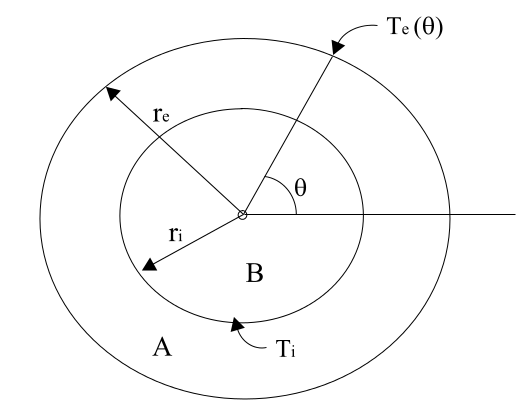
\includegraphics[width=0.6\columnwidth]{imagenes/horno.png}
\caption{Secci\'on circular del horno}
\end{center}
\end{figure}

En el estado estacionario, cada punto de la pared satisface la ecuación del calor:

\begin{equation}\label{calor}
\frac{\partial^2T(r,\theta)}{\partial r^2}+\frac{1}{r}\frac{\partial T(r,\theta)}{\partial r}+\frac{1}{r^2}\frac{\partial^2T(r,\theta)}{\partial \theta^2} = 0
\end{equation}

\medskip

Para resolver este problema computacionalmente, discretizamos el dominio del problema (el sector A) en coordenadas polares. Consideramos una partici\'on $0 = \theta_0 < \theta_1 < ... < \theta_n = 2\pi$ en $n$ \'angulos discretos con $\theta_k-\theta_{k-1} = \Delta\theta$ para $k = 1,...,n$, y una partici\'on $r_i = r_0 < r_1 < ... < r_m = r_e$ en $m+1$ radios discretos con $r_j - r_{j-1} = \Delta r$ para $j = 1,...,m$.

\medskip

El problema ahora consiste en determinar el valor de la funci\'on $T$ en los puntos de la discretizaci\'on $(r_j,\theta_k)$ que se encuentren dentro del sector A. Llamemos $t_{jk} = T(r_j,\theta_k)$ al valor (desconocido) de la funci\'on $T$ en el punto $(r_j,\theta_k)$.

\medskip

Para encontrar estos valores, transformamos la ecuaci\'on (\ref{calor}) en un conjunto de ecuaciones lineales sobre las inc\'ognitas $t_{jk}$, evaluando (\ref{calor}) en todos los puntos de la discretizaci\'on que se encuentren dentro del sector A. Al hacer esta evaluaci\'on, aproximamos las derivadas parciales de $T$ en (\ref{calor}) por medio de las siguientes f\'ormulas de diferencias finitas:


\begin{equation}
\frac{\partial^2T(r,\theta)}{\partial r^2}(r_j,\theta_k) \cong \frac{t_{j-1,k}-2t_{jk}+t_{j+1,k}}{(\Delta r)^2}
\end{equation}

\begin{equation}
\frac{\partial T(r,\theta)}{\partial r}(r_j,\theta_k) \cong \frac{t_{j,k}-t_{j-1,k}}{\Delta r}
\end{equation}

\begin{equation}
\frac{\partial^2T(r,\theta)}{\partial \theta^2}(r_j,\theta_k) \cong \frac{t_{j,k-1}-2t_{jk}+t_{j,k+1}}{(\Delta \theta)^2}
\end{equation}


\subsection{Representación del sistema}

Para representar el sistema de ecuaciones presentado, se utilizará una matriz simple, implementada como un vector de vectores. A continuación, se muestra como quedaría la matriz para las ecuaciones de los puntos $t_{0,0}, t_{0,n-1}, t_{i,j}, t_{m,0}$ y $t_{m,n-1}$.

\[
    % reduce columns padding:
    \setlength{\arraycolsep}{1pt}
    % fila vertical alternativa:
    % \vdots   &  \multicolumn{6}{c}{\strut}      &\vdots&         \multicolumn{6}{c}{}               & \vrule & {} \\
    \kbordermatrix{%
                       & \bm{t_{0,0}} & \ldots & \bm{t_{0,n-1}} & \ldots & t_{i-1,j}           & \ldots & t_{i,j-1}   & \bm{t_{i,j}}                & t_{i,j+1}   & \ldots & t_{i+1,j}   & \ldots & \bm{t_{m,0}} & \ldots & \bm{t_{m,n-1}} &        & b        \\
        \bm{t_{0,0}}   & 1            & \ldots & 0              & \ldots & 0                   & \ldots & 0           & 0                           & 0           & \ldots & 0           & \ldots & 0            & \ldots & 0              & \vrule & t_{0,0}   \\
        \vdots         & \vdots       & {}     & \vdots         & {}     & \vdots              & {}     & \vdots      & \vdots                      & \vdots      & {}     & \vdots      & {}     & \vdots       & {}     & \vdots         & \vrule & {}       \\
        \bm{t_{0,n-1}} & 0            & \ldots & 1              & \ldots & 0                   & \ldots & 0           & 0                           & 0           & \ldots & 0           & \ldots & 0            & \ldots & 0              & \vrule & t_{0,n-1} \\
        \vdots         & \vdots       & {}     & \vdots         & {}     & \vdots              & {}     & \vdots      & \vdots                      & \vdots      & {}     & \vdots      & {}     & \vdots       & {}     & \vdots         & \vrule & {}       \\
        \bm{t_{i,j}}   & 0            & \ldots & 0              & \ldots & \bm{\beta - \gamma} & \ldots & \bm{\alpha} & \bm{-2\alpha-2\beta+\gamma} & \bm{\alpha} & \ldots & \bm{\beta}  & \ldots & 0            & \ldots & 0              & \vrule & 0        \\
        \vdots         & \vdots       & {}     & \vdots         & {}     & \vdots              & {}     & \vdots      & \vdots                      & \vdots      & {}     & \vdots      & {}     & \vdots       & {}     & \vdots         & \vrule & {}       \\
        \bm{t_{m,0}}   & 0            & \ldots & 0              & \ldots & 0                   & \ldots & 0           & 0                           & 0           & \ldots & 0           & \ldots & 1            & \ldots & 0              & \vrule & t_{m,0}   \\
        \vdots         & \vdots       & {}     & \vdots         & {}     & \vdots              & {}     & \vdots      & \vdots                      & \vdots      & {}     & \vdots      & {}     & \vdots       & {}     & \vdots         & \vrule & {}       \\
        \bm{t_{m,n-1}} & 0            & \ldots & 0              & \ldots & 0                   & \ldots & 0           & 0                           & 0           & \ldots & 0           & \ldots & 0            & \ldots & 1              & \vrule & t_{m,n-1}
    }
\]

Donde,
\begin{itemize}
    \item $\alpha = \frac{1}{(\Delta\theta)^2 * r^2}$
    \item $\beta = \frac{1}{(\Delta\ r)^2}$
    \item $\gamma = \frac{1}{(\Delta\ r) * r}$
    \item $0 < i < n$
    \item $0 < j < m+1$
\end{itemize}

\medskip

Notese que la ecuación del punto $t_{i,j}$ tiene ceros en todas sus celdas, excepto en las corresponiendentes a $t_{i-1,j}$, $t_{i,j}$, $t_{i+1j0}$, $t_{i,j-1}$ y $t_{i,j+1}$.
Se puede ver que para cada fila de la matriz, hay una ``banda'' de tamaño $2n$ alrededor de la diagonal donde hay 5 elementos que no son cero.
